%%%% ijcai17.tex

\typeout{IJCAI-17 Instructions for Authors}

% These are the instructions for authors for IJCAI-17.
% They are the same as the ones for IJCAI-11 with superficical wording
%   changes only.

\documentclass{article}
% The file ijcai17.sty is the style file for IJCAI-17 (same as ijcai07.sty).

\usepackage{ijcai17}
\usepackage{CJK}  
\usepackage{url}
% Use the postscript times font!
\usepackage{times}
\usepackage{bm}
\usepackage{graphicx}
\usepackage{amsmath}
\usepackage{amssymb}
\usepackage{xcolor}
\usepackage{xspace}
\newcommand{\todo}[1]{\textcolor{red}{TODO: #1}\PackageWarning{TODO:}{#1!}}
\newcommand{\red}[1]{\textcolor{red}{#1}}
\newcommand{\blue}[1]{\textcolor{blue}{#1}}
\newcommand{\yellow}[1]{\textcolor{yellow}{#1}}
\newcommand{\green}[1]{\textcolor{green}{#1}}
\newcommand{\cyan}[1]{\textcolor{cyan}{#1}}
\newcommand{\brown}[1]{\textcolor{brown}{#1}}
\newcommand{\purple}[1]{\textcolor{purple}{#1}}
\newcommand{\orange}[1]{\textcolor{orange}{#1}}

% the following package is optional:
%\usepackage{latexsym} 

% Following comment is from ijcai97-submit.tex:
% The preparation of these files was supported by Schlumberger Palo Alto
% Research, AT\&T Bell Laboratories, and Morgan Kaufmann Publishers.
% Shirley Jowell, of Morgan Kaufmann Publishers, and Peter F.
% Patel-Schneider, of AT\&T Bell Laboratories collaborated on their
% preparation.

% These instructions can be modified and used in other conferences as long
% as credit to the authors and supporting agencies is retained, this notice
% is not changed, and further modification or reuse is not restricted.
% Neither Shirley Jowell nor Peter F. Patel-Schneider can be listed as
% contacts for providing assistance without their prior permission.

% To use for other conferences, change references to files and the
% conference appropriate and use other authors, contacts, publishers, and
% organizations.
% Also change the deadline and address for returning papers and the length and
% page charge instructions.
% Put where the files are available in the appropriate places.

\title{Predicting Appropriate Charges of Chinese Criminal Cases Based on Fact Descriptions}
%\author{Carles Sierra\\ 
%Artificial Intelligence Research Institute, IIIA-CSIC, Bellaterra, Catalonia  \\
%pcchair@ijcai-17.org}

\begin{document}
\begin{CJK*}{UTF8}{gbsn}  

\maketitle

\begin{abstract}
In this paper, we investigate the problem of determining the appropriate charges for a certain case under the circumstance of statutory law. This problem is important when users communicate with legal assistance systems with natural language, since we need to first determine the category of the case before giving any useful responses. We propose that judgement documents of statutory law countries like China provides natural training data for this task and we find that model multi-label document classification technics fit this problem well. Furthermore, we also find that using additional information of law articles can further improve the model performance in the system of statutory law.
\todo{polish the abstract}
\end{abstract}
\section{Introduction}
The task of automatic charge prediction is to determine appropriate charges, 
such as \emph{fraud}, \emph{larceny} or \emph{homicide},  for a given case by analyzing its 
textual fact description.  Such techniques are crucial for legal assistant systems, where
users could find similar cases or possible penalties by describing a case with their own words,
% \orange{This kind of systems are helpful for people who have no legal background and know nothing about the legal jargon, since extra support from the legal professionals are usually expensive.}
even they have no legal background and 
know nothing about the legal jargon, \orange{since extra support from the legal professionals are usually expensive.}

%Determining appropriate charges, such as \emph{fraud}, \emph{larceny} or \emph{homicide}, 
%based on the fact description of a case is one of the key components in legal assistance systems.
% when the user would like to query the system by describing the case, and it is \orange{even more important} when the user has no idea of the legal basis of a case, where the only input he (or she) can give is the fact description of the case. 
% In this situation, predicting appropiate charges would help us to provide the user with relevant  
%For example, if the user wants to find similar cases, one can use the predicted charges of the query case to filter out irrelevant results. And if the user wants to know the possible penalties \orange{regarding a case}, one also need to decide appropriate charges first.



%In these situations, we need to predict appropirate charges based solely on the fact descriptions of a case. 
However, predicting appropriate charges based on fact descriptions is not trivial:
(1) The differences between two charges can be subtle, for example, in the context of criminal cases in China, 
distinguishing \emph{intentional homicide} from \emph{intentional injury} would require to determine, 
from the fact description, whether the defendant  \textit{intended to kill} the victim, 
or just \textit{intended to hurt the victim, who, unfortunately, died of his severe injury}.
%but in the cases where the victim is dead.
% distinguishing \emph{intentional homicide} from \emph{negligent homicide} would require detailed analysis of the behavior of the defendant.
% and \emph{acceptance of bribes} differs from \emph{acceptance of bribes by a non-state functionary} in the occupation of the defendant. 
(2) Multiple crimes may be involved in a single case, which means that we need to conduct charge prediction in the multi-label classification paradigm. 
(3) Although we can expect an off-the-shelf classification model to learn to label a case with corresponding charges % certain judgement tags %  implicitly learn the legal basis of the judgement 
through massive training data,  it is always more convincing to make the prediction with its involved law articles explicitly shown to the users, as \orange{certain} legal basis to support the prediction. % judgement.  
%the predicted charges are still not convincing enough if no law articles are involved in the prediction. 
This issue is of great importance in countries using \textit{the civil law system}, e.g., China (except Hong Kong) and Germany, where the judgement is made based on statutory laws only. 
For example, in Figure \ref{fig_example_case}, a judgement document in China always includes relevant law articles (usually in the court view part) to support the final decision.  
Even in countries using \textit{the common law system}, e.g., the United States (except Louisiana) and the United Kingdom, where the judgement is based mainly on decisions of previous cases, there are still several statutory laws that need to be followed when making decisions. 

% Therefore, to solve this problem, we need a multi-label classification model, that can effectively capture the overall \orange{framework} along with important details of the fact description, and is able to extract and utilize relevant law articles to build the bridge from the fact description to appropriate charges as well. 

Existing attempts formulate the task of automatic charge prediction as a single-label classification problem, 
by either adopting a k-Nearest Neighbor (KNN)~\cite{LIU2004case,liu2006exploring} as the classifier 
with \orange{simple textual features},
% \orange{with carefully selected feature templates}, 
% or manually designing rules to identify key factors \red{to recognize} specific charges~\cite{lin2012exploiting}, 
or manually designing key factors for specific charges to help text understanding~\cite{lin2012exploiting},
which make those works unable to scale to more types of charges. 
%Previous works on charge prediction either use k-Nearest Neighbor (KNN)~\cite{LIU2004case,liu2006exploring} as classifier or need to manually design key factors of specific charges \cite{lin2012exploiting}, thus do not scale well with regard to data size and number of charges. Furthermore, none of them consider the situation where multiple charges are involved. 
There are also works addressing a related task, finding the law articles that are involved in a given case.
% There are also works addressing a related task, finding specific law articles that has been violated in a 
% given case%~\cite{liu2005classifying,liu2006exploring}
% \red{, which can be considered as a subtask to find legal basis to support the charge prediction task}.  
A simple solution is to convert  this multi-label problem 
into a multi-class classification task by only considering a fixed set of article 
combinations~\cite{liu2005classifying,liu2006exploring}, which
%On the other hand, \cite{liu2005classifying,liu2006exploring} also try to find the specific law articles that has been violated, but converts the multi-label problem into multi-class classification by only considering a fixed set of article combinations, therefore 
can only be applied to a small set of articles and does not fit to real applications.  
%scale to the situation when a larger set of articles are involved. 
Recent improvement takes a two-step approach by performing 
 % \cite{liu2015predicting} aims to find relevant articles in a scalable way by doing
a preliminary classification first and then reranking the results with word-level and article-level features~\cite{liu2015predicting}. 
%Although the framework is promising, only shallow, i.e., word-level, semantic features are employed in their work. 
These efforts  advance the applications of machine learning and natural language processing methods into legal assistance services, however, they are still in an early stage, e.g., relying on expert knowledge, % expert-designed rules, 
using relatively simple classification paradigms, and shallow textual analysis. More importantly, related tasks, e.g., charge prediction and relevant article extraction,  are 
% \red{currently} 
treated independently, 
%Furthermore, all of these works treat charge prediction and article prediction separately, 
ignoring the fact that they could benefit from each other.  


% Since the judgement of a case often involves deciding appropriate charges, our work is part of the thread of work that tries to predicting the results of a case. Previous works on this thread mainly focuses on a binary classification paradigm. The target is either to decide whether the outcome will side with the plaintiff or defendant~\cite{aletras2016predicting}, or will the justice or the present court affirm or reverse the decision of a lower court~\cite{lauderdale2014scaling,sim2015utility,katz2016general}. Except for their binary prediction nature, these methods either do not use fact descriptions or just capture shallow semantic meaning of the facts, e.g., using Bag-of-Words (BOW). Furthermore, although \cite{aletras2016predicting} also tries to use relevant law articles for prediction, the articles they use are gold standard ones while we extract the relevant article by ourselves.
% Therefore, these methods are not suitable for our task. 

% \footnote{\cite{katz2016general} also use an additional \emph{other} class to represent other complex outcomes.}

% To make conprehensive understanding of the fact description, \orange{we propose to use the framework of the Hierarchical Attention Network (HAN)} \cite{yang2016hierarchical} for document embedding. Specifically, we use a sentence-level and a document-level Gated Recurrent Unit (GRU) to embed each word and each sentence along with their contexts. 

Recent advances in neural networks enable us to jointly model charge prediction and relevant 
article extraction in a unified framework, %which enables them to influence each other \orange{in a positive way}.
where the latent correspondence from the fact descriptions about a case to its related law articles 
and further to its charges can be explicitly addressed by a \orange{two-stack attention} mechanism.
Specifically,   %to understand the \orange{whole framework} of the facts, inspired by previous works on document classification \cite{tang2015document,yang2016hierarchical}, 
we use a sentence-level and a document-level Bi-directional Gated Recurrent Units (Bi-GRU)~\cite{bahdanau2015neural} \orange{with a stack of fact-side attention modules} to model the associations among words and sentences, in order to capture \orange{the whole story as well as important details of the case}.  
%To capture the important details, we use attention mechanism to select the most informative words or sentences for sentence and document embedding respectively. 
%To handle the multi-label nature of the problem, we convert the multi-label target to label distribution, and then use cross entropy as loss function. 
% We find this method works well in our experiments and significantly outperforms the baseline BOW method.
Given the analysis about the fact descriptions, we accordingly learn \orange{a stack of article-side attention modules} to attentively select the most supportive law articles from the statutory laws  to support our charge prediction, which is investigated in a multi-label paradigm.
%we first use a simple BOW-based article classifier to quickly \orange{filter out most of the irrelevant articles}. 
%Then we attentively aggregate the retained top $k$ articles for further charge classification.
% Although the top $k$ articles are noisy, the experimental results show that our attentive aggregation module can further attend to relevant ones and thus improve the prediction performance. 

We evaluate our model in the context of  predicting charges for criminal cases in China. 
We collect publicly available judgement documents from China's government website, 
from which we can automatically extract 
% which can be automatically annotated \orange{with}  
%Since the public judgement documents often contain 
\textit{fact descriptions}, \textit{relevant law articles} and \textit{the charges} using simple rules, as shown in Figure~\ref{fig_example_case}.
%, we use rules and regular expressions to extract these information and build a dataset accordingly. 
Experimental results show that our neural network method can effectively predict appropriate charges for a given case, and also provide relevant law articles as legal basis to support the prediction. Our experiments also confirm that, apart from providing legal basis, relevant articles also contain \orange{useful information} that can help to improve charge prediction in \orange{the civil law system}.
%Furthermore, since there exist differences between the words used by laymen and legal practitioners, 
We also examine our model on the news reports about criminal cases composed by journalists.
%and the results show that, 
Although trained on judgement documents, our model can still 
\orange{achieve promising performance on news data, showing a reasonable generalization ability over different expression styles.} 
% \red{achieve a F1 score of 79.12\% on news data,  with 20\% less performance drop compared to baselines,
% (Just say, achieve promising performance???)
% showing a better generalization ability in more diverse situations. 
% (This expression is not good, same for Section 5.4)}


% our method significantly outperforms the baselie BOW-based Suport Vecotr Machine (SVM) method, and the automatically extracted relevant law articles can clearly improve the model with only facts as input. 
% We also find that our model can effectively attend to the true relevant articles, which to some extent provides us with the legal basis for our charge prediction. 

% In this paper, we focus specifically on predicting the charges of criminal cases in China, \orange{which began to} officially publish the judgement documents on China Judgements Online\footnote{http://wenshu.court.gov.cn/} since 2013. Although these judgement documents are unstructured, we can use rules and regular expressions to extract the facts description, relevant law articles, and final charges of the case. This naturally provides us with a high-quality large-scale training dataset for our task.

% \red{TO REMOVE:}
% The contributions of this paper are threefold: 
% (1) It proposes a novel neural network model that can jointly utilize the facts and the automatically extracted relevant law articles of a case to predict appropriate charges.
% (2) The proposed model can also provide legal basis for the charge prediction in the form of weighted relevant law articles.
% (3) By further evaluating the model on human labeled news data, it shows that, although trained on judgement documents, the proposed model also has reasonable generalization ability on the text written by people who are not legal practitioners.


\begin{figure*}[t!]
\begin{center}
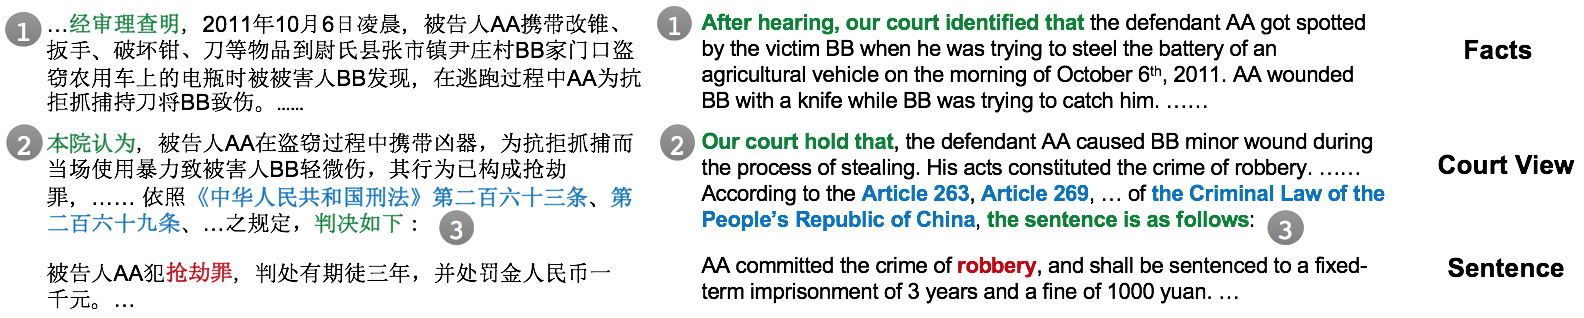
\includegraphics[width=0.97\textwidth]{figures/case.png}	
\caption{An example judgement document excerpt of a criminal case in our dataset. Names are anonymized as AA and BB.
Rectangulars, ellipses and dashed rectangulars refer to the clauses that usually indicates the bedinning of the facts part, the court view part and the decision part, respectively. Articles and charges are extracted with regular expressions and a charge list.
}
\label{fig_example_case}
\end{center}
\end{figure*}

\section{Related Work}
\label{sec_related_work}
The charge prediction task aims at predicting appropriate charges based on the facts of a case.
\cite{LIU2004case,liu2006exploring} use KNN to classify charges of criminal cases in Taiwan. However, except for the inferior scalability of the KNN method, their word-level or phrase-level features also do not provide enough information to distinguish very similar charges. 
\cite{lin2012exploiting} proposes to make deeper understanding of a case by identifying charge-specific factors manually designed for two charges. Their method also suffers from sclability issue due to the human efforts requied to design and annotate these  factors. Our method, however, employs GRU and attention mechnism to make comphrehensive understanding of a case, and all the training data are automatically constructed based on public judgement documents. 

On the other hand,
\cite{liu2005classifying,liu2006exploring} also try to find the specific law articles that has been violated. However, they convert the multi-label problem to multi-class classification problem by only considering a fixed set of article combinations, which cannot scale well since the number of possible combinations will grow expentially when a larger set of law articles are considered.
\cite{liu2015predicting} instead designs a scalable way to find relevant law articles, 
by first using Support Vector Machine (SVM) for preliminary article classification, and then 
rerank the results by using the similarity between the words in facts and articles, and the correlations among law articles as indicators.
% use some reranking methods to get the final relevant article list. 
We also utilizes SVM to extract top $k$ articles, but instead use GRU and attention mechanism to better understand the texts and the correlation among articles.
% However, to better understand the association between facts and articles, we use attention mechanism to distinguish relevant ones in the top $k$ extraction results. \orange{To make our model fully differenciable,} rather than using frequent pattern mining techinque, we use RNN to model the correlations among articles.

Another related thread of work in field of artificial intelligence and law is to predict the overall outcome of a case. The target can be predicting which party will the outcome side with~\cite{aletras2016predicting}, or will the present court affirm or reverse the decision of a lower court~\cite{katz2016general}. Our work mainly differs from them in that, instead of binary outcome (the latter one also contains an \emph{other} class), we step further to focus on the detailed results of a case, i.e., the charges, where the output may contain multiple labels. 

% Another related thread of work is to predict the overall outcome of a case. The target can be predicting whether the outcome will side with the plaintiff or defendant~\cite{bruninghaus2003predicting,aletras2016predicting}, or will the present court affirm or reverse the decision of a lower court~\cite{martin2004competing,katz2016general}. Our work mainly differs from them in that, instead of binary outcome, we step further to focuse on the detailed results of the case, i.e., the charges, where the output may contain multiple labels. 


We share similar spirit with the legal question answering task~\cite{COLIEE14}, which aims at answering the yes/no questions in Japanese legal bar exams, that we all believe that relevant law articles are important for decisions in civil law system. 
The task requires participants to first extract relevant Japanese Civil Code articles, and then use them to answer the questions. 
The article extraction phase is often treated as an information retrieval task, and the question answering phase is usually considered as a textual entailment task~\cite{kim2014legal,kimconvolutional}
% Another thread of work also tries to answer the multiple-choice questions in the USA National Bar Exam \cite{FAWEI16,adebayoneural}. Since the United States mainly operates on common law system, where statutory laws are less important, the relevant article extraction phase is not employed in these works.

Our work is also related to the task of document classification, but differs from it in that we also use automatically extracted law articles to improve and support the charge prediction.
% , a simple but effective method is to combine bag-of-words (BOW) features with varies classifiers~\cite{joachims1998text}. 
Recently, neural network (NN) models like Convolutional Neural Network (CNN)~\cite{kim2014convolutional} have been used for document embedding, and the resultant document vecotr is further used for classification.
\cite{tang2015document} proposes a two-layer scheme, where they use recurrent neural network (RNN) or CNN for sentence embedding, and another RNN for document embedding.
Our method also uses this two-layer scheme, and shares similar spirit with \cite{yang2016hierarchical} in using context vectors to distinguish informative words or sentences from non-informative ones, but instead of global context vectors, we allow them to be dynamically generated for each datum when extra guidance is available.
% We also differs from these works in using extracted relevant law articles to support charge classification, which require us to distinguish relevant articles from irrelevant ones, and further aggregate the information from two sources for classification.

As for multi-label classification, two loss functions are commonly used in natural language processing. 
The first one is binary cross entropy~\cite{nam2014large}, which treats the multi-label classification task as multiple binary classification tasks. 
The second one is cross entropy~\cite{kurata2016improved}, which converts the multi-label target to label distribution during training, and use a threshold selected on validation set to generate the final prediction during testing. In our pilot experiments, we find the latter one converges faster and performs better, so the latter one is used in this paper.
\section{Data Preparation} 
Our data are collected from the website of China Judgements Online. The Chinese government has been publishing the judgement documents on it since 2013.
% \footnote{There are also judgements before 2013.}. 
We randomly choose 50,000 judgements as training data, 5,000 for validation and 5,000 for test. To ensure enough training data for each charge, we only keep the charges that appear more than 50 times in the training data. As for law articles, we only consider the ones in the Criminal Law of the People's Republic of China. The resulting dataset contains 50 distinct charges and 321 distinct articles. About 3.56\% cases contain more than one charges, and 94.18\% cases contain more than one law articles. \orange{An average case has 1.03 charges and 3.81 law articles}. The fact description part of each judgement document contains 382.60 words, and 14.21 sentences on average.

An example judgement is shown in Figure \ref{fig_example_case}. Although there does not exist a strict rule for formatting a judgement document, we can still discover some patterns in it. A typical judgement document often starts with a brief description of the \emph{procedure} \orange{followed before the judgement}, from the start of the prosecution until the case is decided. The procedure part is often followed by the \emph{facts} of the case. After that, the court will conclude the case and provide relevant law articles that can be applied to the case (\emph{court view}). Finally, the \emph{sentence} part will list the charges of the defendant along with the corresponding penalties. 

We find that the fact description part often starts with the clause 经审理查明$\ $(after hearing, our court identified that), the court view part often starts with the clause 本院认为$\ $(our court hold that), and the sentence part often starts with the clause 判决如下$\ $(\orange{the sentence is as follows}). Therefore we extract the texts between these two clauses as fact description, and consider the text after 判决如下$\ $as sentence part. Since the charge mentions do not have many variations in judgement documents, we manually build a list that contains the possible variations of each charge based on a public criminal charge list\footnote{\url{http://china.findlaw.cn/zuiming/}}. The resulting list is used to find charge mentions in the sentence part with exact matching. As for law articles, since the article is often mentioned in a fixed patterns, we simply use regular expressions
% \footnote{``第[、零〇一二两三四五六七八九十百千0-9]+条(之[一二两三四五六七八九十])?)''} 
to identify the article mentions. 

Note that we only retain the cases with one defendant. Because in the situation with multiple defendants, it is hard to separately relate each defendant to his (or her) corresponding facts, articles and charges due to the unstructured nature of the judgement document.

\begin{figure}[t!]
\begin{center}
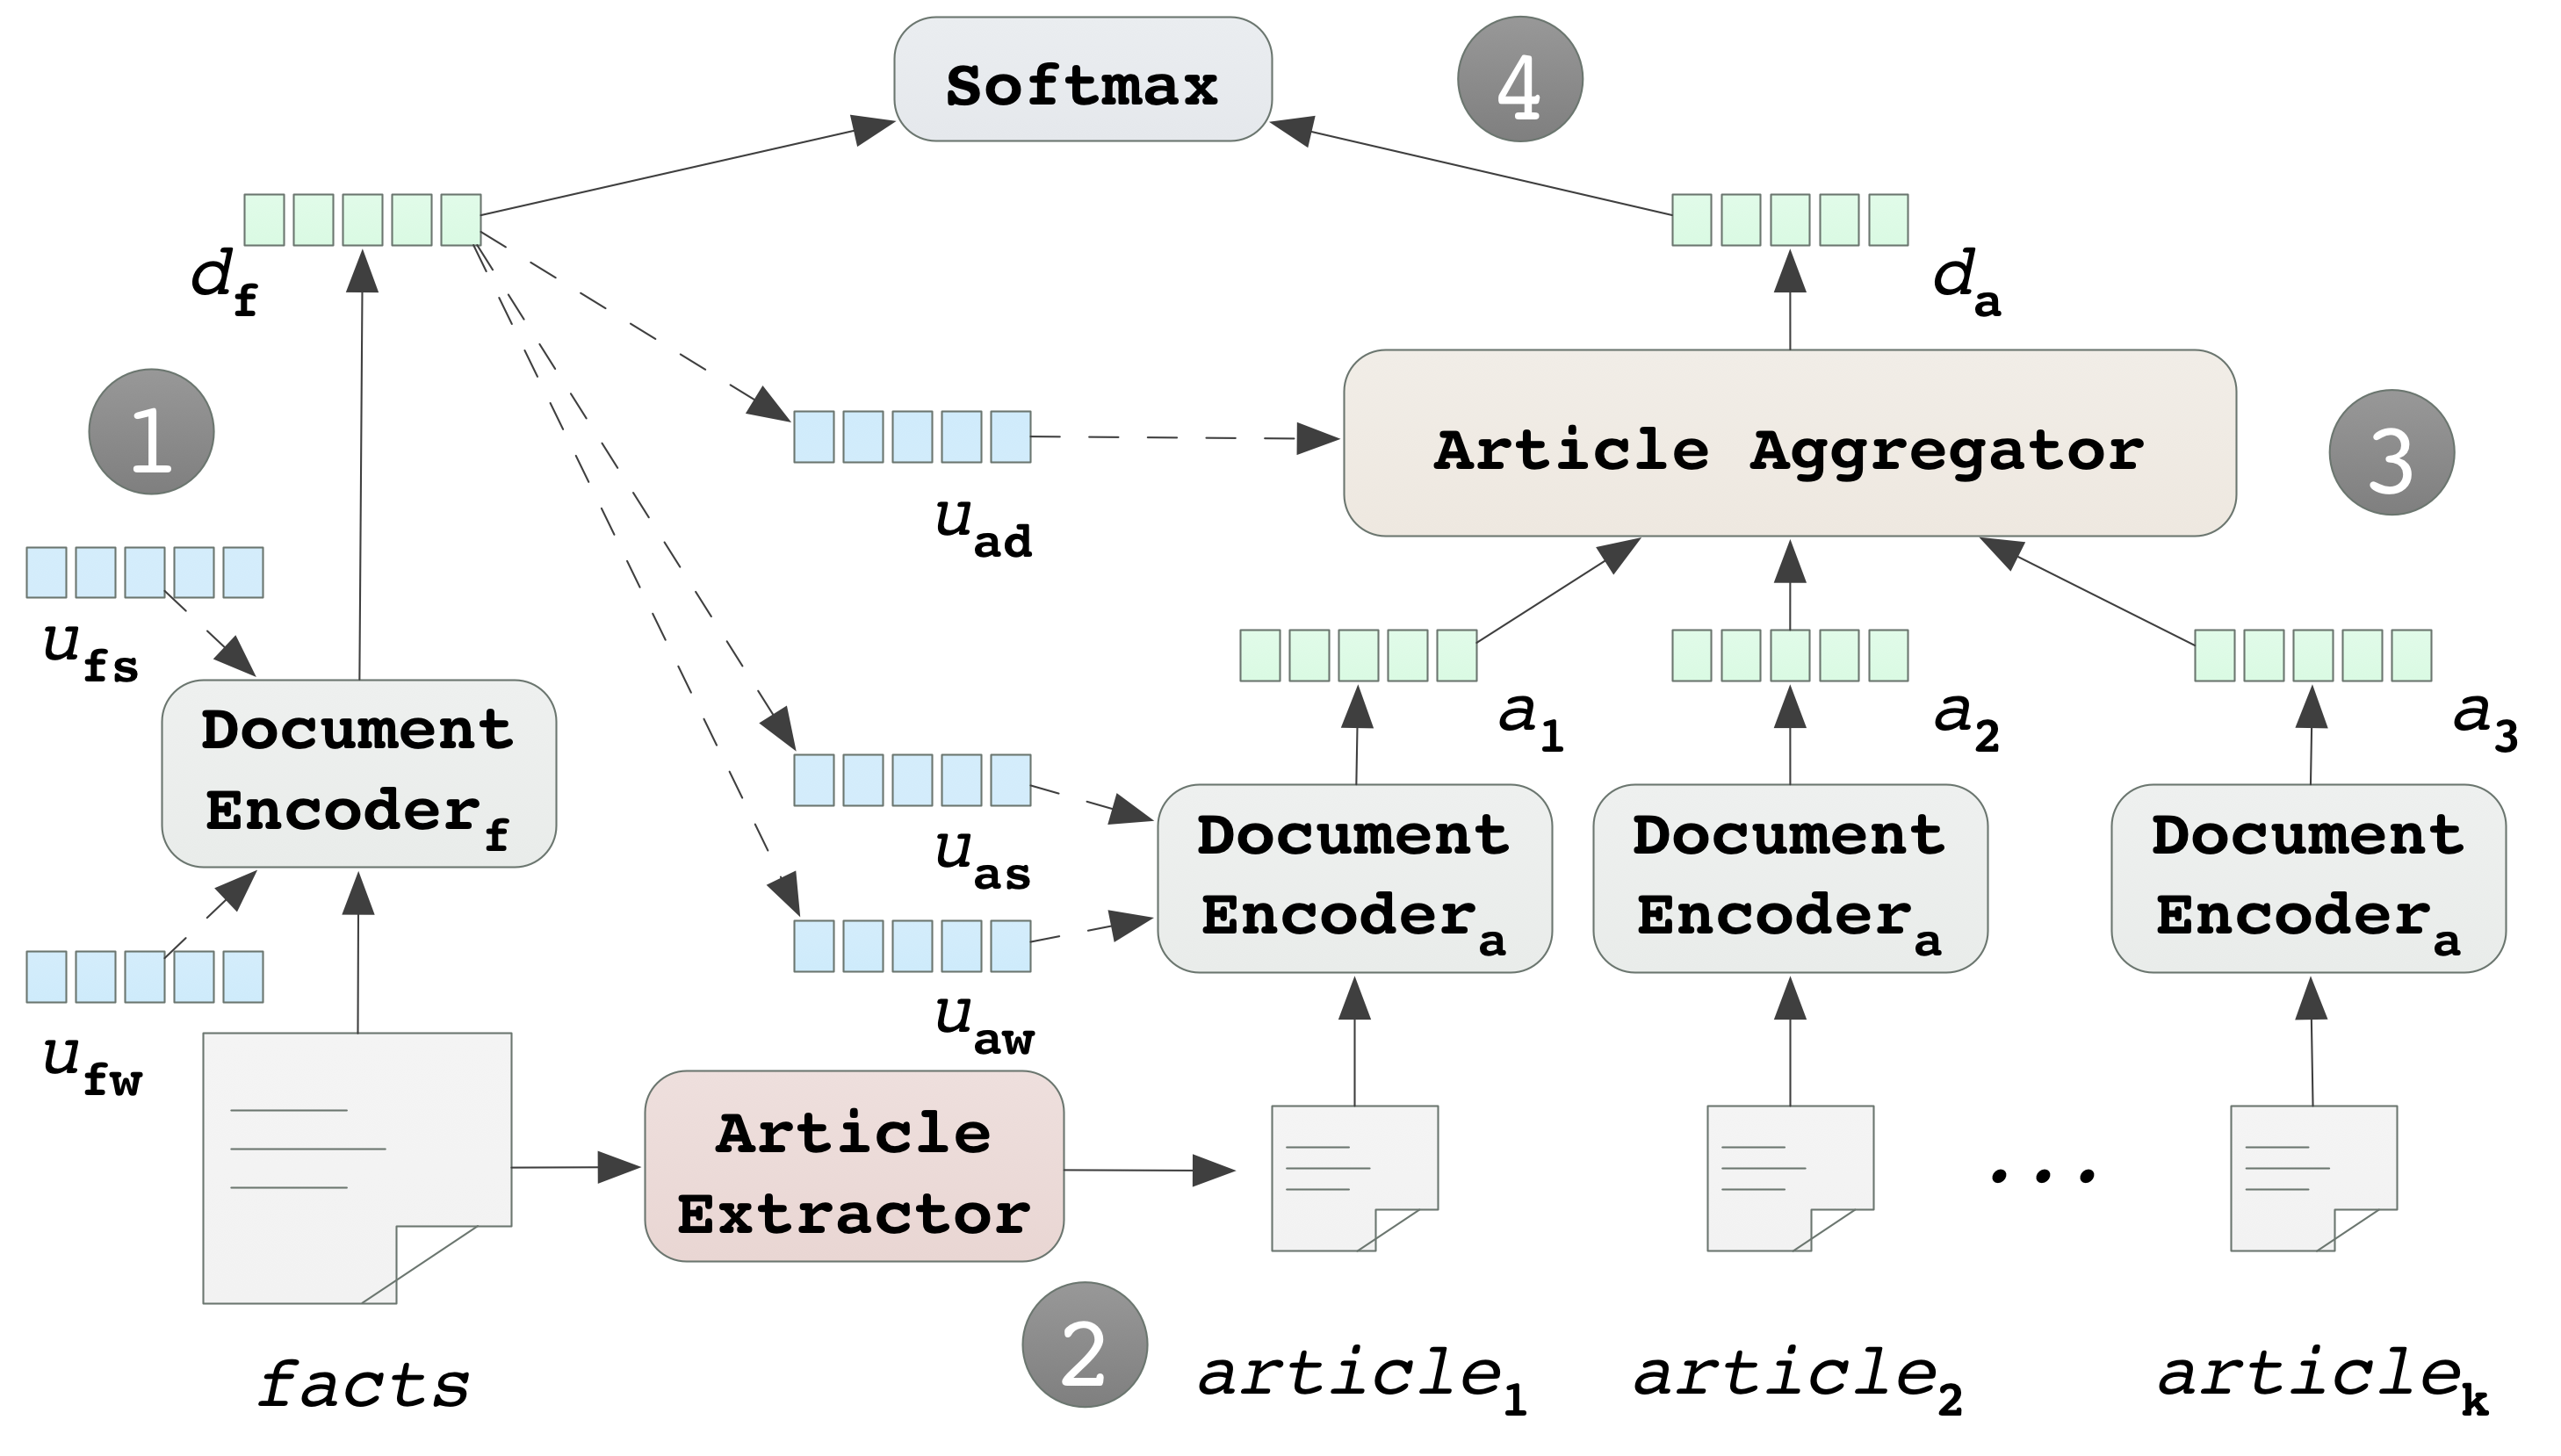
\includegraphics[width=0.48\textwidth]{figures/charge_pred_overview.png}	
\caption{Overview of Our Model}
\label{fig_model_framework}
\end{center}
\end{figure}

\section{Our Approach}
In order to generate reasonable charge prediction, our approach follows four steps as depicted in Figure \ref{fig_model_framework}. 
(1) The input fact description is fed to a document encoder to generate the fact embedding $\mathbf{d_f}$.
(2) Concurrently, the input fact description is also passed to a relevant article extractor to find top $k$ relevant law articles. 
(3) Each article is fed to another document encoder, and the article embeddings are further passed to an article aggregator to produce the aggregated article embedding $\mathbf{d_a}$. Meanwhile, three global context vectors, i.e., $\mathbf{u_{aw}}$, $\mathbf{u_{as}}$ and $\mathbf{u_{ad}}$, are generated from the fact embedding $\mathbf{d_f}$ for the document encoder and the article aggregator. 
(4) Finally, $\mathbf{d_f}$ and $\mathbf{d_a}$ are concatenated and passed to a softmax classifier to predict the charge distribution of the input case.
\orange{what is the best way to organize this section?}

%The fact-based charge classification task can be formatted as a multi-label document classification task. The input is several sentences describing the facts of a case, and the output is multiple charges related to the case. Since usually multiple elements are required to constitute a charge (for example, the charge of acceptance of bribes requires the defendant to illegally accepts another person's money, and the defendant should also be a state functionary), the recurrent neural network (RNN) seems like a natural fit for the task. Considering the fact that only a small portion of the facts are crucial for the determination of charges, we also use attention mechanism in our model. Since the HAN model  satisfies many of our requirements except the multi-label classification capability, we use the framework of the HAN model for document embedding, but replace the output module and the loss function with ones that are compatible with the multi-label classification task. Furthermore, to take the information of article into account, we add another article attention module to incorporate the information of relevant articles to the model.

\subsection{Document Encoder}
\label{sec_doc_encoder}
% Our document encoder module is based on the framework of Hierarchical Neural Network (HAN) proposed by \cite{yang2016hierarchical}. The overview of our document encoder is shown in Figure \ref{fig_doc_encoder}. 
Intuitively, a sentence is a sequence of words and a document is a sequence of sentences. As suggested by previous works \cite{tang2015document,yang2016hierarchical}, the document embedding problem can be converted to two sequence embedding problems, i.e., embedding sequence of words and embedding sequence of sentences. Therefore, the key problem of document embedding lies in building an effective sequence encoder. As shown in Figure \ref{fig_doc_encoder}, we can first generate the embedding of each sentence using the sentence-level sequence encoder, and then aggregate these sentences embeddings with document-level sequence encoder to generate the document embedding $\mathbf{d}$. Although it is possible to use different models for these two sequence encoders, we simply use the same architecture here for simplicity.

\begin{figure}[htbp]
\begin{center}
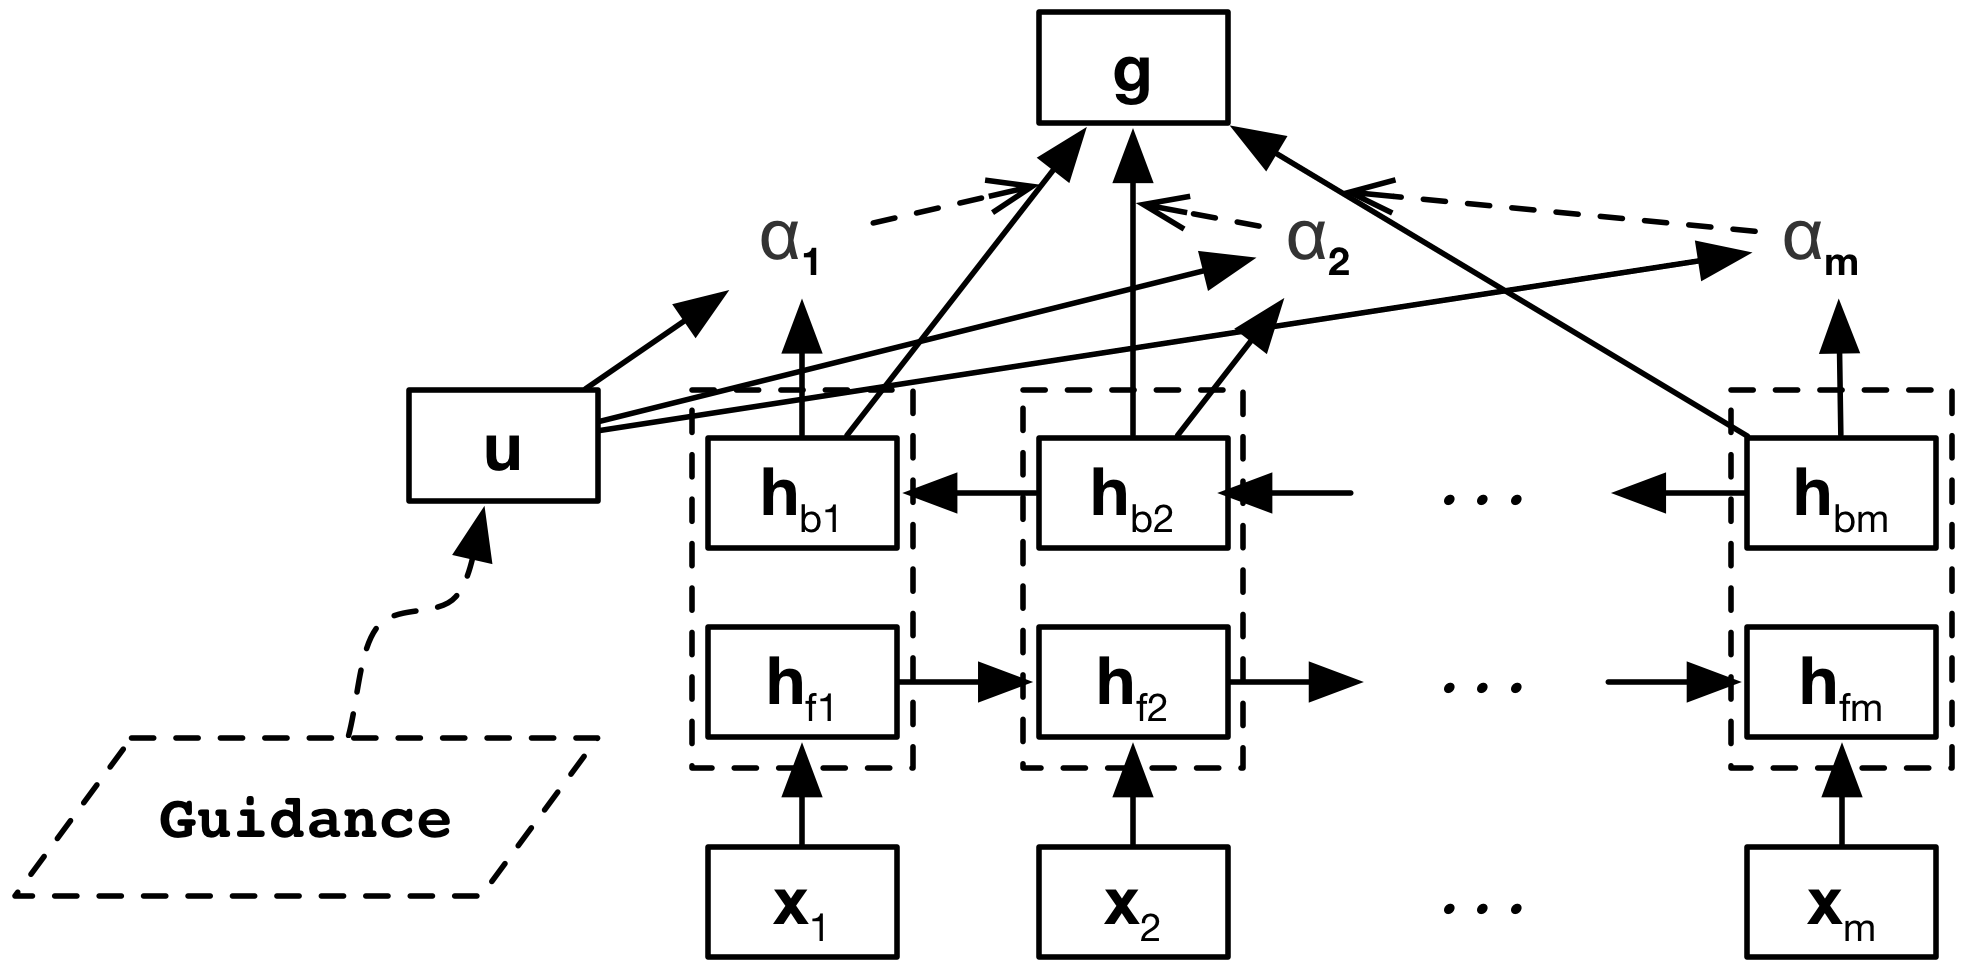
\includegraphics[width=0.45\textwidth]{figures/attentive_seq_encoder.png}	
\caption{Attentive Sequence Encoder}
\label{fig_seq_encoder}
\end{center}
\end{figure}

\begin{figure}[htbp]
\begin{center}
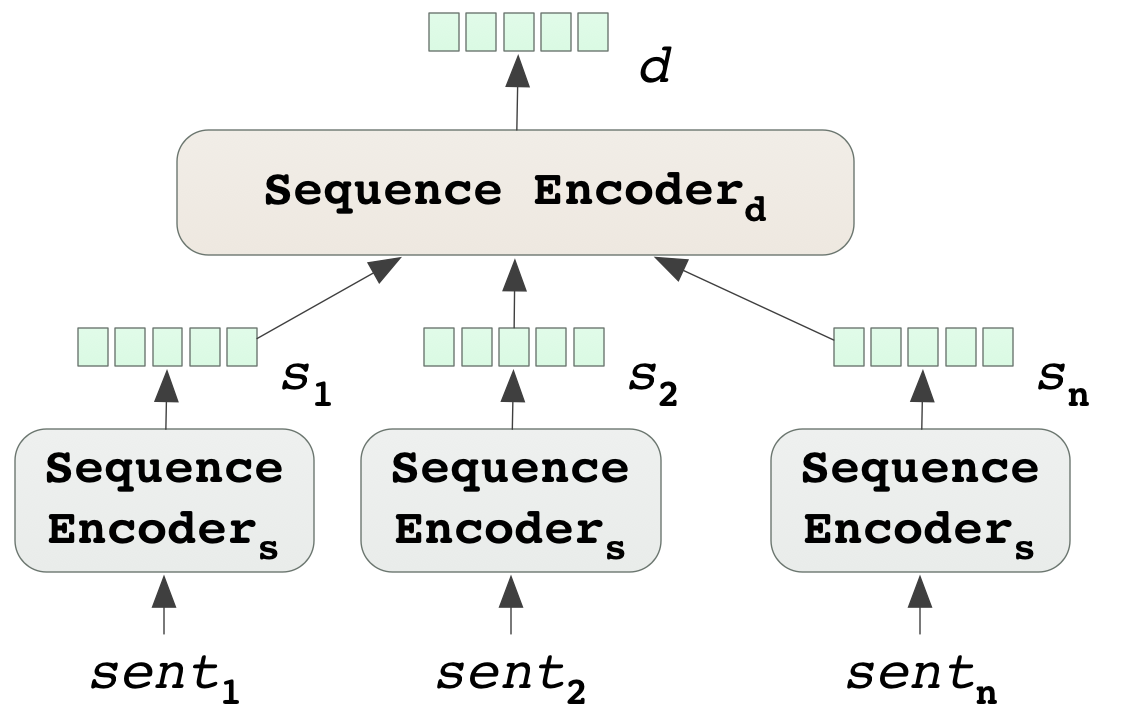
\includegraphics[width=0.4\textwidth]{figures/document_encoder.png}	
\caption{Document Encoder}
\label{fig_doc_encoder}
\end{center}
\end{figure}

\paragraph{Bi-GRU Sequence Encoder} 
One of the key challenges in building a sequence encoder is how to take the correlation of each elements into consideration. A promising solution is the bi-directional gated recurrent unit (Bi-GRU) model proposed by \cite{bahdanau2015neural}, which encodes the context of each element by using a gating mechanism to track the state of sequence.
Specifically, the Bi-GRU model first uses a forward and a backward GRU~\cite{cho2014learning}, which a kind of Recurrent Neural Network (RNN), to encode the sequence in two opposite directions, and then concatenate the results of both GRUs to form the final outputs. 

Given a sequence $[\mathbf{x}_1, \mathbf{x}_2, ..., \mathbf{x}_T]$ where $\mathbf{x}_t$ is the input embedding of the element at position $t$, the state of Bi-GRU at position $t$ is:

\begin{equation}
%h_t = [\overrightarrow{h}_t , \overleftarrow{h}_t]
\mathbf{h}_t = [\mathbf{h}_{ft}, \mathbf{h}_{bt}]
\end{equation}
where $\mathbf{h}_{ft}$ and $\mathbf{h}_{bt}$ are the state the forward and backward GRU at position $t$ respectively. 

% And the state of a single GRU (take forward GRU as an example) is calculated by:
% \begin{equation}
% \mathbf{h}_{ft}=(1-z_t)\odot \mathbf{h}_{f,t-1} + z_t\odot \tilde{\mathbf{h}}_{ft}
% \end{equation}

% \begin{equation}
% \tilde{\mathbf{h}}_{ft}=tanh(\mathbf{W}_h \mathbf{x}_t + r_t\odot \mathbf{U}_h \mathbf{h}_{f,t-1} + \mathbf{b}_h)
% \end{equation}

% \begin{equation}
% r_t=\sigma(\mathbf{W}_r \mathbf{x}_t + \mathbf{U}_r \mathbf{h}_{f,t-1} + b_r)
% \end{equation}

% \begin{equation}
% z_t=\sigma(\mathbf{W}_z \mathbf{x}_t+\mathbf{U}_z \mathbf{h}_{f,t-1} + b_z)
% \end{equation}
% where $\tilde{\mathbf{h}}_{ft}$ is the candidate state of position $t$, $z_t\in{[0,1]}$ is the update gate, $r_t\in{[0,1]}$ is the reset gate, $\mathbf{W}$ and $\mathbf{U}$ are weight matrices, $b$ is the bias, $\odot$ represents element wise product and $\sigma$ corresponds to the sigmoid function. The final sequence embedding is either the concatenation of $\mathbf{h}_{fT}$ and $\mathbf{h}_{b1}$, or simply the average of the average of $\mathbf{h}_t$.

\paragraph{Attentive Sequence Encoder}
\label{sec_att_seq_encoder}
However, $[\mathbf{h}_{fT}, \mathbf{h}_{b1}]$ often fails to capture the whole semantic meaning when the sequence is long, and using the average of $\mathbf{h}_t$ also has the drawback that it treats useless elements equally with informative ones. 

In similar spirit with \cite{yang2016hierarchical}, we also use a global context vector to attentively aggregate the elements in the sequence, but we further allow the global context vector to be dynamically generated when extra guidance is available (see Section \ref{sec_article_encoder}).


The framework of our attentive sequence encoder is show in Figure \ref{fig_seq_encoder}. Given the Bi-GRU output sequence $[\mathbf{h}_1, \mathbf{h}_2, ..., \mathbf{h}_T]$, we calculate a sequence of attention values $[\alpha_1, \alpha_2, ..., \alpha_T]$ where $\alpha_t \in [0, 1]$ and $\sum_t{\alpha_t}=1$. The final embedding of the sequence is calculated by:
\begin{equation}
\mathbf{g} = \sum_{t=1}^{T}{\alpha_t \mathbf{h}_t}
\label{seq_embed}
\end{equation}
where the attention value $\alpha_t$ is calculated by:
\begin{equation}
\mathbf{v}_t = tanh(\mathbf{W} \mathbf{h}_t)
\label{eq_att_transform}
\end{equation}
\begin{equation}
\alpha_t=\frac{exp(\mathbf{v}_t^T \mathbf{u})}{\sum_t{exp(\mathbf{v}_t^T \mathbf{u})}}
\label{gen_att}
\end{equation}
where $\mathbf{W}$ is a weight matrix, and $\mathbf{u}$ is the global context vector that is used to distinguish informative elements from non-informative ones. 


\subsection{Using Law Articles}
One of the difficulties of using law articles to support our charge prediction lies in the fact that statutory laws contain a large number of law articles, which makes complex classification models time-consuming in training, and run slowly in \orange{production environment} as well. 

Therefore, we propose a two-step approach to resolve this problem. Specifically, at the first step, we use a fast and easy-to-scale classifier to filter out a large fraction of irrelevant articles, and retain the top $k$ articles for the next step. Then, we use neural network to make more conprehensive understanding of the top $k$ articles, and use attention mechanism to select the most relevant ones for charge classification.

\paragraph{Top $k$ Article Extractor}
\label{sec_article_extractor}
We consider the relevant article extraction task as multiple binary classification tasks. Specifically, since 321 distinct law articles in the Criminal Law of the People's Republic of China are mentioned in our dataset, we therefore build 321 binary classifiers where each classifier focuses on the relevance of a specific law article. Moreover, if more articles are considered (e.g. articles in the Anti-Drug Law of the People's Republic of China), we can simply add more binary classifiers accordingly, with the existing classifiers untouched.

We use bag-of-words-based Support Vector Machine (SVM) as our binary classifier, which is fast and performs well in text classification~\cite{joachims2002learning,wang2012baselines}. Specifically, we use bag-of-words TF-IDF features, chi-square for feature selection and SVM with linear kernel for binary classification. The articles are ranked by the score output by SVM and the top $k$ articles are kept for each judgement document.

\paragraph{Article Encoder}
\label{sec_article_encoder}
We use neural network method to make deeper understanding of the extracted top $k$ articles. 
As shown in Figure \ref{fig_model_framework}, each article is first passed to a document encoder to generate the article embedding $\mathbf{a}_j, j\in [1, k]$. 
While using similar architecure, this document encoder differs from the one used for fact embedding that, instead of using global context vectors, the word-level and sentence-level context vectors, i.e., $\mathbf{u_{aw}}$ and $\mathbf{u_{as}}$, which are used to produce word-level and sentence-level attention values respectively, are generated dynamically for each case from the fact embedding $d$:
\begin{equation}
\mathbf{u}_{aw} = \mathbf{W}_w \mathbf{d} + \mathbf{b}_w
\end{equation}
\begin{equation}
\mathbf{u}_{as} = \mathbf{W}_s \mathbf{d} + \mathbf{b}_s
\end{equation}
where $\mathbf{W}$ is the weight matrix and $\mathbf{b}$ is the bias. The dynamic context vectors enables us to attend to informative words or sentences with respect to each specifica case, rather than just selecting \orange{generally informative ones}.

\paragraph{Attentive Article Aggregator}
The article aggregator aims to generate an aggregated embedding of the top $k$ articles, and the difficulty lies in how to attend more to relevant articles while ignore the irrelevant ones. 

Due to the inferior classification ability of the relevant article extractor, the order of the top $k$ articles are not \orange{very meaningful}. Therefore, the top $k$ articles are more of a set rather than a sequence. However, as suggested by \cite{vinyals2016matching}, when encoding a set, it is still beneficial to use a bi-directional RNN to embed the context of each element.
In our task, specifically, using bi-directional RNN is beneficial to model the co-existence tendency of among relevant articles.

Therefore, we use the attentive sequence encoder described in Section \ref{sec_att_seq_encoder} to generate the aggregated article embedding $\mathbf{d}_a$. To attend to the relevant articles, we also dynamicall generate the context vector $\mathbf{u}_{ad}$ by:
\begin{equation}
\mathbf{u}_{ad} = \mathbf{W}_d \mathbf{d} + \mathbf{b}_d
\end{equation}


\subsection{Output and Loss Function}
To generate the charge prediction, we first concatenate the document embedding $\mathbf{d}_f$ and the aggregated article embedding $\mathbf{d}_a$, and feed them to two full connection layer to generate a new vector $\mathbf{d}$. Then, $\mathbf{d}$ is passed to a softmax classifier to generate the predicted charge distribution. We use the validation set to determine a threshold $\tau$, and consider all the charges with a output probability higher than $\tau$ as positive predictions.

% Note that although other multi-label classification paradigms are also applicable to our problem (see Section \ref{sec_related_work}), we use this method because it performs best in our pilot experiments. 
Also note that the input to the first full connection layer can also be $\mathbf{d}_f$ only, which meanings we do not use the information from relevant law articles (see comparison in Section \ref{sec_main_results}). 

As for training, we use cross entropy as our loss function:
\begin{equation}
\label{original_loss}
Loss= -\sum_{i=1}^N\sum_{l=1}^L{y_{il} log(o_{il})}
\end{equation} 
where $N$ is the number of training data, $L$ is the number of charges, $y_{il}$ and $o_{il}$ are the target and predicted probability of charge $l$ of datum $i$. Here the target charge distribution $\mathbf{y}$ is generated by setting positive labels to $\frac{1}{m}$ and negative labels to $0$, where $m$ is the number of positive labels.

\paragraph{Guided Article Attention}
Note that each judgement document also contains gold standard law articles that can be applied to this case. Therefore, we can use this information to guide the attention of the attentive article aggregator during training. Specifically, given the $k$ articles, we want the article attention distribution $\bm{\alpha}=[\alpha_1, \alpha_2, ..., \alpha_k]$ to simulate the target distribution $\mathbf{t}\in\mathbb{R}^k$: \todo{can be simplified}
\begin{equation}
t_j=
\begin{cases}
1/|\mathbb{A}|,	& j\in \mathbb{A}\\
0,	& else
\end{cases}
\end{equation}
where $\mathbb{A}$ is the set of indices of the gold standard articles in the top $k$ extracted articles, and $|\mathbb{A}|$ is the size of set $\mathbb{A}$. 

Therefore, the final loss function is:
\begin{equation}
\label{final_loss}
Loss = -\sum_{i=1}^N(\sum_{l=1}^L{y_{il} log(o_{il})} + \beta \sum_{j=1}^k{t_{ij} log(\alpha_{ij})})
\end{equation}
where $\beta$ is the weight vector used to control the importance of article attention guidance.


% There are two commonly used methods for multi-label classification in neural network models. The first one is to consider the multi-label classification problem with $L$ labels as $L$ binary classification problem. It uses sigmoid function in the output layer and binary cross entropy as loss function. This method performs well in many multi-label text classification problems \cite{nam2014large}.

% The second method uses the softmax function to generate outputs. It first convert the multi-label target to a probability distribution. For example, suppose there are 4 classes and one datum belongs to class 0 and class 2. This method will convert the $y=[1, 0, 1, 0]$ to $y=[0.5, 0, 0.5, 0]$, and cross entropy will be used as the loss function. After training, a threshold $\tau$ is selected and all the classes that have a score higher than $\tau$ will be considered as positive classes. This method proves to work well in the natural language query classification task \cite{kurata2016improved}. 

% In our pilot experiments, we find that the first method converges about 5 times slower than the second method in our dataset, and the second method also produces better results. We think this phenomenon happens because only a small fraction of our data are multi-label data. Therefore the second method, which uses the same output function as multi-class classification tasks, works better in our task. In this paper, we will use the second method.
\section{Experiments}
\subsection{Experimental Setup}
We use HanLP\footnote{\url{https://github.com/hankcs/HanLP}} for Chinese word segmentation and POS tagging.
Word embeddings are trained using word2vec~\cite{mikolov2013distributed} on judgement documents, web pages from several legal forums and Baidu Encyclopedia. The resulting word embeddings contain 573,353 words, with 100 dimension.
% We use word2vec~\cite{mikolov2013distributed} to train our word embeddings with judgement documents, and web pages from several legal forums as well as Baidu Encyclopedia. The resulting word embeddings contain  573,353 words, with 100 dimension.  
%As for word embeddings, we use Baidu Encyclopedia, 3 million judgement documents and 3 million legal question answer pairs crawled from multiple legal forums as corpus, and the word2vec~\cite{mikolov2013distributed} for training. 
%The size of the resultant word embedding is 100-d and there are 573,353 words in total. 
% During training and testing, all the time expressions, names and charges\footnote{Although rare, sometimes the charge may appear in the fact part. This conversion ensures that we do not use this information.} in the text are converted to 3 special tokens separately and the words not in the pre-trained word embeddings are converted to another special token. All the word embeddings remain unchanged during training except for the special tokens. 
We randomly initialize a 50-d vector for each POS tag, which is concatenated with the word embedding as the final input.
Each GRU in the Bi-GRU is of size 75, the two full connection layers are of size 200 and 150.
The relevant article extractor generates top 20 articles, the weight of the article attention loss ($\beta$ in Eq.~\ref{final_loss}) is 0.1, and prediction threshold $\tau$ is 0.4.
We use Stochastic Gradient Descent (SGD) for training, with learning rate 0.1, and batch size 8.
% We also clip the gradient so that the sum of square of the L2 norms of the trainable tensors does not exceed 5. 
% To accelerate the training, we constrain the number of sentences of each fact description to be less than 50 and the the maximum length of each fact sentence to be 50. As for articles, we constrain the maximum length of each sentence to be 30. 
%The chi-square feature selector keeps the top 2,000 features.
% , and we use the SVM model implemented in scikit-learn \cite{scikit-learn} in our experiments.

We compare our full model with two variations: without article attention supervision and only using facts for charge prediction. We also implement an SVM model, which proves to be effective in \orange{many text classification tasks}~\cite{wang2012baselines,aletras2016predicting}. Specifically, the SVM model takes bag-of-words TF-IDF features as input, and uses chi-square to select top 2,000 features.


\begin{table}
\centering
\small{
\begin{tabular}{|c|c|c|c|}
\hline
% \multirow{2}{|c|}{Model} & \multicolumn{3}{c|}{\tabincell{c}{ (\textit{Micro-/Macro-}) }}
\multirow{2}{*}{\textbf{Model}}				& \tabincell{c}{\textbf{Precision}} 	& \tabincell{c}{\textbf{Recall}} 		& \tabincell{c}{\textbf{F1}} 	\\
% \hline
\cline{2-4}
                                               & \multicolumn{3}{c|}{\tabincell{c}{ (\textit{Micro-/Macro-}) }}\\
\hline
\textit{SVM} 				& \textbf{93.94}/79.53					& 77.66/49.54  					& 85.03/61.05 				 	\\
\hline
\textit{SVM\_article} 			& 91.77/71.33					& 72.10/45.85  					& 80.76/55.82				 	\\
\hline
\textit{NN}				& 91.30/\textbf{83.32}			& 87.39/74.99  					& 89.31/78.94					\\
\hline
\textit{NN\_article\_only} 			& 90.09/81.50				& 86.10/69.62				& 88.05/75.10		\\
\hline
\textit{NN\_article}			& 90.79/83.07					& 88.42/75.73  					& 89.59/79.23					\\
\hline
\textbf{\textit{NN\_supv\_article}} 	& 91.80/82.44 					& \textbf{88.67/78.62} 			& \textbf{90.21/80.48} 		 	\\
\hline
\hline
\textit{SVM\_gold\_article$^*$} 	& \textbf{98.97}/94.58			& 95.39/83.21  					& 97.15/88.53					\\
\hline
% \textit{SVM\_only\_gold$^*$} 		& 98.78/90.46					& 97.92/91.79  					& 98.35/91.12					\\
% \hline
\textbf{\textit{NN\_gold\_article$^*$}} 		& 98.78/\textbf{95.26} 			& \textbf{98.24/95.57} 			& \textbf{98.51/95.42} 			\\
\hline
% \hline
% \textit{NN\_article\_only} 			& 90.09/81.50				& 86.10/69.62				& 88.05/75.10		\\
% \hline
% \textit{NN\_gold\_only$^*$} 		& 97.22/92.39				& 98.36/94.73				& 97.79/93.55		\\
% \hline
\end{tabular}
}
% \vspace{-.5em}
\caption{Charge prediction results. $^*$ refers to using gold standard articles during training and testing. Left and right side of the slash refer to micro- and macro-statistics, respectively.}
\label{tabble_main_results}
\end{table}


% \textit{NN\_article\_only} 			& 87.38/78.61				& 82.69/64.32				& 84.97/70.75		\\


\subsection{Charge Prediction Results}
\label{sec_main_results}
%The charge prediction results are summarized in Table \ref{tabble_main_results}. 
% The left side of the slash refers to micro statistics, and the right side refers to macro statistics. 
% Micro precision (or recall) is the the number of correct predictions divided by the total number of predictions (or the total number of gold standard charges), while the macro precision (or recall) is the sum of the precision (or recall) of each charge divided by the number of distinct charges. The micro (or macro) F1 is the harmonic mean of the micro (or macro) precision and recall.
We evaluate the charge prediction task using precision, recall and F1, in both macro- and micro-level.
The macro-precision/recall are calculated by averaging over %the precision/recall of 
each charge, and the micro- ones are averaged  over each prediction. %In other words, macro statistics give equal weight to each charge, while micro statistics give equal weight to each individual prediction. The micro (or macro) F1 is the harmonic mean of the micro (or macro) precision and recall.


%The $Acc.$ refers to instance accuracy, which is the number of instances whose classes are all correctly predicted divided by the total number of instances.

As shown in Table~\ref{tabble_main_results}, %we can see that, 
the basic \texttt{SVM} model,
which only takes fact descriptions as input, indeed proves to be a strong baseline.
By contrast, our corresponding neural network model (\texttt{NN}), which also only uses facts for prediction, outperforms \texttt{SVM} 
by around 4\% in micro-F1.
Since \texttt{NN} benefits from the pre-trained word embeddings,
a two-level Bi-GRU architecture, and the fact-side attention module,
it can thus attentively recognize informative expressions from the description and 
better capture the underlying correspondence from fact descriptions to appropriate charges,
even when there is less overlap in the words used among cases with the same charge,
or when there are limited training data (i.e., infrequent charges). This may also explain that NN models 
have more balanced performance over different charges, leading to more prominent improvements over 
SVM ones in macro metrics, which usually have a strong bias towards frequent charges.
%

%This actually indicates the nature of the civil law system that judgements are made based on statutory laws rather than decisions of previous cases.

When we use both the facts and the extracted relevant law articles (that are admittedly noisy),
the SVM version (\texttt{SVM\_article}) drops by around~5\% than \texttt{SVM}, showing that the SVM model 
cannot benefit from the extracted, thus noisy, relevant articles in such a straightforward way.
However, our NN version (\texttt{NN\_article}) can still learn from  the noisy article extractions through 
attentively aggregating those extracted articles even without direct guidance,
thus improves \texttt{NN} by around 0.4\%.
Furthermore, if we use the gold standard articles during training as supervision for the 
article attention (our full model, \texttt{NN\_supv\_article}), the performance can be further improved, achieving 
90.21\% and 80.48\% in micro- and macro-F1, respectively.
%This proves that it is important to take relevant law articles into considerations for charge prediction.
The improvements made by using relevant law articles actually indicates the nature of the civil law system that judgements are made based on statutory laws rather than decisions of previous cases.

However, if we only use the extracted relevant articles to make prediction (\texttt{NN\_article\_only}\footnote{
\texttt{NN\_article\_only} utilizes fact embeddings to attentively aggregate relevant articles, but only use 
the aggregated article embedding $\mathbf{d}_a$, without fact embedding  $\mathbf{d}_f$,  for charge prediction.}),
even with the proved-helpful attentive aggregator, the model performs worst among all NN 
variants (though still better than \texttt{SVM}). This indicates that  it is necessary to consider both facts and 
relevant law articles for charge prediction, and,
the fact that \texttt{NN} outperforms \texttt{NN\_article\_only} also indicates that although the judgments are made based on the statutory laws in the civil law system,
the \orange{logic of legal reasoning} %\textbf{logical thinking or legal reasoning} 
employed by the court when making decisions,
% of the court behind the formal decisions, 
to some extent, may be implicitly captured through massive fact-charges paris.



\orange{Now the question is: \textit{how much improvement can we have by 
making full use of %expoiting 
the relevant law articles within the civil law system?}}
% \orange{Now the question is: \textit{what is the upper bound of the improvements that can be made by using relevant law articles within the civil law system?}}
Let us consider an ideal situation where we can access both fact descriptions and gold standard law articles during testing, which could be considered as an upper bound scenario.
The SVM version (\texttt{SVM\_gold\_article}) significantly outperforms %\texttt{SVM} by around 27\% in macro-F1, and especial
\texttt{SVM\_article} by more than 30\% in macro-F1.
And the NN version %upper-bound 
(\texttt{NN\_gold\_article}) outperforms 
% our best article version (\texttt{NN\_supv\_article}) 
\texttt{NN\_supv\_article}
by over 8\%.
% , and no surprisingly, \texttt{NN\_article} by more than 10\%.
%
These comparisons confirm again that 
law articles play an important role for automatic judgement prediction, but 
the extracted relevant articles inevitably contain noise, which should be properly 
handled, e.g., using an attentively aggregation mechanism to distill 
valuable evidence to support the charge prediction.



%If we can use both the facts and the gold standard articles of each case during testing (\texttt{SVM\_gold\_article}), the performance will be significantly improved, showing that the relevant law articles contain valuable information for charge prediction. However, the results become worse when we replace the gold standard articles with the extracted ones (\texttt{SVM\_article}), indicating that the simple SVM model cannot benefit from the extracted, thus possibly noisy, relevant articles in a straightforward way. 
% If we only use the gold standard articles of each case for classification (\texttt{SVM\_only\_gold}), the micro F1 can be further improved to 98.35, which further indicates that the SVM model has bad resistence to noise. \todo{is \texttt{\_only\_gold} necessary?}

%On the other hand, since our attentive article aggregator has the ability to distinguish relevant articles from \red{extraction errors/irrelevant ones}, our neural network (NN) model (\texttt{NN\_article}) can learn from  the noisy article extractions, and improve the performance over the model using facts only (\texttt{NN}), which has already outperfoms \texttt{SVM} by a large margin.

%Furthermore, if we use the gold standard articles during training to \orange{supervise} the article attention (\texttt{NN\_supv\_article}), the performance can be further improved.
%Similar to the SVM case, if we can access gold standard articles during testing (\texttt{NN\_gold\_article}),% instead of extracted ones, 
%there will be a clear improvement as well, which actually indicates the upper bound of the improvement that relevant articles can bring to our model.

% and without surprise, it also outperforms \texttt{SVM\_gold\_article}.
%Also note that, compared with the corresponding SVM models, the improvements made by our NN architecture are more prominent in macro statistics, since SVM has a strong bias towards frequent charges, while our NN models have a more balanced improvement in both frequent and infrequent ones. 
%
%Our NN models harness the pre-trained word embeddings \red{with two-stack attention mechanism????} to effectively encode sentences and documents, thus can better capture the underlying correspondence from fact descriptions to appropriate charges, \red{even there is less overlap in the words used, or there are limited training data for infrequent charges.  }
%\orange{This is probably due to the embedding methods used by our NN models. By using pre-trained word embeddings and training effective sentence-level and document-level sequence encoders, our model can capture the meaning of the cases belonging to infrequent charges even if their training data are limited, and thus performs better on these cases.}
% This is probably due to the nature of the BOW feature, which is unable to handle synonyms. However, understanding synonyms is crucial for inferring common patterns when training data are limited. Therefore, by using pre-trained word embeddings to handle synonyms, our NN model perfroms well on infrequent charges. 
% it can better understand the meaning of a word even when it is rare in the training data. 

% As for our neural network (NN) model (\texttt{NN}), since it can better understand the associations among sentences and words, and can select the most informative parts of the text, they significantly outperforms the corresponding SVM models. 

%We also evaluate two variations which only use articles for charge prediction.
%\texttt{NN\_gold\_only} uses concatenated gold standard articles, instead of facts, as input. 
%\texttt{NN\_article\_only} uses extracted articles, and it still uses fact embedding and article aggregator to handle the noise in the top 20 articles, but only the aggregated article embedding $\mathbf{d}_a$ is used for charge prediction.
%We can see that the performance of \texttt{NN\_gold\_only} is very good and \texttt{NN\_article\_only} also generates reasonable results. 
%This actually indicates the nature of the civil law system that judgements are made based on statutory laws rather than decisions of previous cases.
%Also note that \texttt{NN\_gold\_only} is not as good as \texttt{NN\_gold\_article}, showing that the facts can provide additional information for charge prediction even if we use gold standard law articles.
%On the other hand, the performance of \texttt{NN} is also promising and outperforms \texttt{NN\_article\_only}, showing that although the judgments are based on statutory laws, we can still learn the \orange{legal logic} behind this implicitly through only the (facts, charges) paris. 

% Specifically, the relevant articles are concatenated and passed to the model by replacing the fact descriptions. We find that using only the top 20 extracted articles (\texttt{NN\_article\_only}) still generates \orange{fair} results, and the model performs very good when the extracted articles are replaced with gold standard ones (\texttt{NN\_gold\_only}), which significantly outperforms \texttt{NN}. 



% \orange{And the big gap between \texttt{NN\_supv\_article} and \texttt{NN\_gold\_article} indicates that there is still much room that our article extraction and embedding part can improve.}

% Recall that using only facts as input, the results of \texttt{NN} is promising, showing that although the legal system of China is mainly based on civil law system, the judgements are still consistent with the facts enough for our model to implicitly learn the legal logic behind the judgement.
% which to some extent indicates a reasonable consistency of Chinese judges in making judgements. 

\paragraph{Case Study}
We study the model outputs and find certain star-like confusion patterns among the charges. For example, \emph{intentional injury} %(\emph{pivot charges}) 
is often confused with %multiple charges (\emph{peripheral charges}) like 
\emph{intentional homicide} (when the victim is dead, the difference is %it differs from \emph{intentional injury} in
 whether the defendant intends to kill  or just hurt the victim) and \emph{picking quarrels and provoking troubles}
(there may also exist injuries here).
% We refer to charges can be confused with multiple charges as \emph{pivot charges}, and the charge often confused with a single charge as \emph{peripheral charges} here.
These charges usually share similar fact descriptions, e.g., how the injuries are caused, and since \emph{intentional injury} appears more frequently than the others, \texttt{SVM} thus outputs \emph{intentional injury} in most situations, and fails to distinguish these charges.
However, by using Bi-GRU and the attention mechanism, \texttt{NN} can attend to important details of the facts and significantly improves the performance on these charges.
%On the other hand, these learned patterns are not reliable enough, and lead to limited improvements on pivot charges.
When the direct supervision for articles is available,  \texttt{NN\_supv\_article}  can enhance the interaction between certain pairs of descriptions and law articles, which helps to capture the subtle differences among similar charges, and further improves the performance.
%and therefore learns more elaborated patterns, which significantly improve the pivot charges while less prominent improvements on other easily confused charges are made as well.

% On the other hand, while \texttt{NN\_supv\_article} also improves \texttt{NN} on these this kind of charges, a \orange{considerable} amount of improvements comes from the charges that can be confused with multiple charges, e.g., \emph{intentional injury} is also often confused with \emph{picking quarrels and provoking troubles} since there will also be injuries in the latter one, indicating that the additional information from relevant law articles can help the model handle the difficult charges better.


\subsection{Article Extraction Results}
%\paragraph{Top $k$ Article Extraction}
% \begin{table}
% \centering
% \normalsize{
% \begin{tabular}{|c|c|c|c|c|}
% \hline
% 				& \textbf{Top\_5} 	& \textbf{Top\_10} 		& \textbf{Top\_20} 	& \textbf{Top\_30} \\
% \hline
% \textit{Recall} 		& 77.60			& 88.96  				& 94.21			& 96.53 	\\
% \hline
% \textit{NDCG} 		& 80.28			& 84.32  				& 86.47			& 87.24 	\\
% \hline
% \end{tabular}
% }
% \caption{Top $k$ Article Extraction Performance}
% \label{tab_article_extraction}
% \end{table}
We also evaluate our SVM article extractor, which achieves 
%Our top $k$ article extractor achieves 
77.60\%, 88.96\%, 94.21\% and 96.53\% recall regarding the top 5, 10, 20 and 30 articles, respectively.
Although simple, the SVM extractor can obtain over 94\% recall for top 20 articles, which is good enough for further refinement.
However, the micro F1 of the extractor is only 61.08\% in the test set, which will lead to severe error propagation problem if we use them directly. Therefore, we design the article attention mechanism to handle the noise in the top 20 articles.

% Our top $k$ article extractor achieves 94.21\% recall for the top 20 results, which is good enough to for the following refinement components. However, the recall of the top 5 results is 77.60\% and the micro F1 is only 61.08\%, which indicates that we still cannot trust its prediction results directly, and therefore need to expand the number of results to ensure enough recall for the following components. Furtherfore, we find that the recall of the top 30 results is only 2.32\% higher than the top 20 results, therefore we use the top 20 results in this paper.

% Our relevant article extraction module achieves 86.44\% top 1 accuracy, 61.08\% micro F1, and the other evaluation indicators are shown in Table \ref{tab_article_extraction}. 
% We can see that, the relevant article extraction task is also a hard task in itself. Although our SVM model achieves reasonable ranking performance, its prediction performance is not very good. If we use the prediction results directly in our model, we will suffer from a severe error propagation problem. Therefore, we instead let the relevant article extraction module return the top $k$ articles, and use attention mechanism the distinguish true relevant articles from incorrect ones. Since the recall of the top 20 results has achieved 94.21\%, which already includes most of the relevant articles, we use top 20 articles in our experiment.

\begin{table}
\centering
\normalsize{
\begin{tabular}{|c|c|c|c|c|}
\hline
% \textbf{Att\_Weight}
% \bm{$\beta$}
\bm{$\beta$}							& \textbf{Prec@1} 		& \textbf{MAP} 			& \textbf{Charge\_F1} \\
\hline
\textit{0} 								& 60.94								& 61.61 						& 89.59/79.23 	\\
\hline
\textit{0.01} 						& 81.06								& 78.00							& 89.77/79.48 	\\
\hline
\textit{0.1} 							& 87.90								& 83.39							& \textbf{90.21/80.48} 	\\
\hline
\textit{0.5} 							& 91.44								& 86.95							& 89.93/79.67 	\\
\hline
\textit{1} 								& \textbf{92.66}			& \textbf{88.24}		& 89.83/78.66 	\\
\hline
\end{tabular}
}
\caption{Refined Article Extraction Performance}
\label{tab_article_att}
\end{table}


%\paragraph{Article Attention}
We can also evaluate the extracted articles after re-ranking by our article attention module.
%We can consider the article attention module as a re-ranking function over the extracted top $k$ articles, and accordingly use the gold standard articles in the $k$ articles to evaluate the re-ranking performance. 
Table \ref{tab_article_att} shows the refined extraction results  (column 2-3) and the corresponding charge prediction performances (column 4), under different weights for article attention ($\beta$ in Eq.~\ref{final_loss}). \texttt{Prec@1} refers to top 1 precision, and \texttt{MAP} refers to mean average precision.
%
We can see that, even if there is no supervision over the article attention ($\beta=0$), our model still has reasonable performance on re-ranking the $k$ articles. When the attention supervision is employed, the extraction quality improves significantly, and keeps increasing as $\beta$ goes up.
%The \orange{fair} performance of the article attention indicates that our model can provide reasonable legal basis to support the charge prediction.
However, the charge prediction performance does not always increase with the article extraction quality, and the best performance is achieved when $\beta=0.1$. This is not surprising, since  there exists a tradeoff between the benefits of more accurate article extraction and the less model capacity left for charge classification due to the increased emphasis on the article extraction performance.

\begin{table}
\centering
\small{
\begin{tabular}{|c|c|c|c|}
\hline
\textbf{Model}												& \textbf{Precision} 				& \textbf{Recall} 				& \textbf{F1} 	\\
\hline
\textit{SVM} 													& \textbf{100.00}						& 40.20  									& 57.34 				 	\\
\hline
\textit{NN}														& 87.14											& 59.80 									& 70.93					\\
\hline
\textit{NN\_article}					& 87.18											& 66.67 									& 75.56					\\
\hline
\textbf{\textit{NN\_supv\_article}} 	& 90.00 										& \textbf{70.59} 					& \textbf{79.12} 		 	\\
\hline
\end{tabular}
}
\caption{Performance (micro- statistics) on News Data}
\label{tabble_news_results}
\end{table}

\subsection{Performance on News Data}
There are usually 
clear %significant 
differences between the expressions used by legal practitioners and people without legal background, 
thus it is important to see how our model will perform on fact descriptions written by non-legal professionals.
%
%We evaluate our models  on news reports that are composed by general reporters,
%where 
We then manually annotate 100 news reports %by general reporters 
from two news websites\footnote{\url{news.cn/legal} and \url{legal.people.com.cn}},
containing 262 words on average and 25 distinct charges.
%
The results are shown in Table \ref{tabble_news_results}, where we only report micro statistics due to the small size of the dataset.
% since macro ones are not 

%Also note that the size of the news test set is relatively small with regard to the number of charges, which results in less reliable macro statistics, we therefore only report  here.

We can see that, \texttt{SVM} suffers a significant drop in F1 on the news data, %compared to on judgement documents,
confirming the gap between the expressions used by legal practitioners and non-legal professionals,
given the BOW nature of \texttt{SVM}.
Although \texttt{SVM} cannot generalizes well, the patterns learned by \texttt{SVM} are reliable in themselves, leading to a high precision.
It is not surprising that our NN models also suffer from the expression differences, %\orange{news genre}, 
but due to the effectiveness of our NN architecture, with about 10\%$\sim$15\% less absolute drop in F1, and \texttt{NN\_supv\_article} can still achieve 79.12\% in F1. %, \orange{thanks to our NN architectures}.
%exists a performance drop, they are much better than the SVM model. This shows that the  gap in expressions can be resolved by using embedding methods to a some extent. 
For example, the word 暴打$\ $(beat up) is seldom used in judgement documents,
making it hard for \texttt{SVM} to correctly utilize  暴打$\ $as an indicator for injury related charges, but, %However, by using pre-trained word embeddings, 
our NN models can associate it with its  near-synonymy  殴打$\ $(beat), which is a formal expression in judgement documents.
Furthermore, the clear improvements from \texttt{NN} to \texttt{NN\_article}, and further to \texttt{NN\_supv\_article} prove again the importance of relevant articles 
in supporting charge prediction, even in news domain.
%we can see that the model using relevant articles (\texttt{\_article}) clearly outperforms \texttt{NN}, \orange{showing that relevant articles also provide valuable information in this situation.}

% Also note that, since the news test set is relatively small regarding the number of charges, the macro statistics are not as meaningful as those in the judgement document test set. For example, correctly predicting a charge with only one instance will improve the macro precision and recall by 4\% (${1}\div{25}$). Therefore, \texttt{NN\_article} outperforms \texttt{NN\_supv\_article} in macro F1 by 4.38\% does not necessarily mean that it performs better on infrequent charges. 
% Actually, %except for other differences, 
% \texttt{NN\_article} only generates one more such case than \texttt{NN\_supv\_article}, while \texttt{NN\_supv\_article} correctly predicts 4 more cases than \texttt{NN\_article} in total. Therefore, we still consider \texttt{NN\_supv\_article} to be better than \texttt{NN\_article} on news data.


% Also note that compared with \texttt{NN\_article}, \texttt{NN\_supv\_article} has better micro statistics but worse macro statistics, indicating that the additional supervision over article attention makes the model perform better on frequent charges but worse on infrequent ones on news data. 
% The reason is that, since the top $k$ article extractor also utilizes BOW features, its performances drops significantly on news data, leading to some situations where the key article is not included in the top $k$ results. While the attention of \texttt{NN\_article} will be diffusive in these situations, due to the article attention supervision, \texttt{NN\_supv\_article} has a stronger tendency to put the attention on the articles related to frequent or other relevant charges, and thus is more likely to generate false prediction.  
% \todo{re-organize this part}


\section{Conclusion}
In this paper, we propose an attention based neural network framework that can jointly model the charge prediction and the relevant article extraction task, where the weighted relevant articles can serve as legal basis to support the charge prediction.
The experimental results on judgement documents of Chinese criminal cases show the effectiveness of our model on both charge prediction and relevant article extraction.
The comparison of different variants of our model also indicates the importance of law articles in making judicial decisions in the civil law system.
By experimenting on news data, we show that, although trained on judgement documents, our model also has reasonable generalization ability on fact descriptions written by non-legal professionals.
While promising, our model still cannot explicitly handle multi-defendant cases, and there is also a significant gap between our model and the upper bound improvement that relevant articles can achieve. We will leave these challenges for future work.


% In this paper, we investigate the problem of predicting appropriate charges of a case given only the fact descriptions as input. We argue that relevant law articles provide valuable information for charge prediction, and accordingly propose an attention based neural network model to jointly utilize the facts and the automatically extracted law articles for charge prediction. The weighted relevant law articles generated by our model can also be considered as legal basis of the prediction. By evaluating our model on the judgement document data, we find our model significantly outperforms the SVM model, and relevant articles can clearly improve the model with only facts as input. The experiments on news data further show that, although trained on judgement document data, our model has reasonable generalization ability on the fact descriptions written by people who are not legal practitioners.

\clearpage
%% The file named.bst is a bibliography style file for BibTeX 0.99c
\bibliographystyle{named}
\bibliography{ijcai17}

\end{CJK*}  
\end{document}

